\chapter{Análisis}
% Planeacion del sistema
% Siguiente capitulo: Primer prototipo - Desarrollo Frontend
%   - Analisis
%   - Diseno
%   - etc...

\section{Alcance}

La magnitud de este problema abarca a todos los organismos, direcciones o cualquier dependencia del Instituto Politécnico Nacional. Aunque la solución puede escalar a todo el instituto y su marco normativo, el alcance de este proyecto \textit{considerará únicamente a la comunidad de la Escuela Superior de Cómputo y a los reglamentos con mayor relevancia para las actividades académicas}. Para ello, en este proyecto, inicialmente contará con los siguientes 

\begin{itemize}
    \item Ley Orgánica
    \item Reglamento Interno
    \item Reglamento de Titulación
    \item Reglamento General de Estudios
\end{itemize}

\section{Requerimientos Funcionales}

A continuación, se describe el comportamiento y la funcionalidad esencial para que el chatbot pueda cumplir el objetivo:

\begin{enumerate}[leftmargin=2.5cm ,label={\bfseries RF-\arabic*}]
    \item \label{itm:consultar-reglamento} Un usuario de esta aplicación debe poder consultar un segmento de los documentos del marco normativo en cualquiera de los siguientes niveles de división estructural del documento:
    \begin{itemize}
        \item título
        \item capítulo
        \item sección
        \item artículo.
    \end{itemize}
    
    \item La aplicación debe manejar una conversación de manera lógica (i.e., responder adecuadamente a la conversación en los temas a las preguntas referentes al marco normativo).
    \item \label{itm:requisito-intenciones} El chatbot debe poder detectar si la intención del mensaje es alguno de los siguientes:
        \begin{itemize}
            \item Saludar.
            \item Solicitar información de un articulo.
            \item Solicitar artículos relacionados a una situación en particular.
            \item Despedir.
        \end{itemize}
    \item El chatbot debe saludar de acuerdo a la hora del día.
    \item El chatbot debe poder identificar las entidades o conceptos que el usuario solicita consultar.
    \item \label{itm:rf-servicio-web} La aplicación debe ser disponible a través de un servicio web.
    \item  \label{itm:cliente-web} La aplicación debe proporcionar un cliente accesible a través de un navegador web.
\end{enumerate}

\section{Requerimientos No Funcionales}

\begin{enumerate}[leftmargin=2.5cm ,label={\bfseries RNF-\arabic*}]
    \item Se sugiere que el resultado de las consultas sean breves y concisos. 
    \item El bot debe poder expresar intenciones de asesorar en temas referentes al marco normativo.
    \item Se desea que la aplicación se desarrolle utilizando herramientas de licencia abierta y software libre.
\end{enumerate}


\section{Metodología}

Las actividades a desarrollarse se harán siguiendo una metodología de \textbf{prototipado evolutivo}. Esta elección se hace con base a la necesidad de estar tener que estar evaluando constantemente el diseño inicial de la funcionalidad, principalmente la ejecución del algoritmo de similitud. Para ello, se busca poder refinar detalles sin perder la estabilidad de las iteraciones pasadas.

Los prototipos están basado en los siguientes componentes:

\begin{itemize}
    \item \textbf{Interfaz de usuario}: contiene la página web y el sistema cliente que se encarga de realizar peticiones HTTP al chatbot.
    \item \textbf{Base de conocimiento}: serialización y persistencia del conocimiento de los documentos normativos y su representación semántica necesaria para poder procesarla.
    \item \textbf{Intérprete semántico}: componente de entendimiento del chatbot que se encarga de procesar consultas textuales en búsquedas de similitud sobre la base de conocimiento.
    \item \textbf{Preprocesador de Texto}: contiene todos los ejecutables y las implementaciones de los algoritmos que ayudan a transformar documentos de un formato a otro para la extracción, transformación de datos necesarios para el intérprete y carga a la base de conocimiento.
\end{itemize}

\begin{figure}
    \centering
    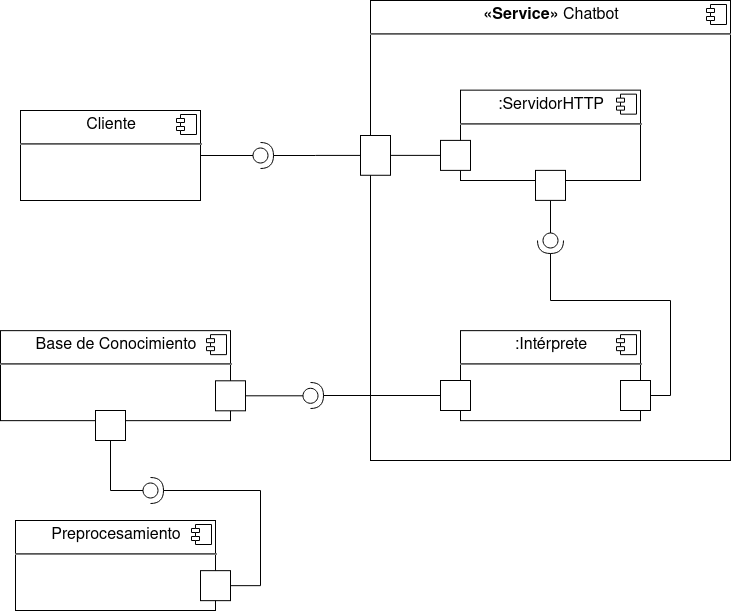
\includegraphics[scale=0.5]{images/4/componentes}
    \caption{Diagrama de componentes}
    \label{fig:diagrama-componentes}
\end{figure}

\subsection{Primer Prototipo}

En este primer prototipo inicial se espera construir el componente visual del  cliente web así como la preparación de los datos a procesar y la definición inicial del esquema en la fuente de datos. Las actividades principales en esta etapa son:

\begin{itemize}
    \item Construcción de la página web
    \item Desarrollo del sistema cliente
    \item Construcción del servicio de almacenamiento
\end{itemize}

\subsection{Segundo Prototipo}

En este segunda iteración del prototipado se enfocará principalmente a la implementación del intérprete que categoriza la intención de un usuario, así como las funciones que se encargarán de gestionar el procesamiento de la acción correspondiente a la intención.

\begin{itemize}
    \item Implementación del intérprete con reconocimiento de intención.
    \item Algoritmos de transformación de texto.
\end{itemize}

\subsection{Tercer Prototipo}

Para este punto, se esperaría cumplir con los requerimientos de manera suficiente para cumplir el objetivo. Por lo tanto, en esta etapa la integración de todos los componentes y poder tener un flujo funcional del sistema completamente integrado.

\begin{itemize}
    \item Integración del algoritmo de similitud de conceptos.
    \item Integración de la funcionalidad de recuperación de artículos de la base de datos.
\end{itemize}

\subsection{Futuras iteraciones}

Una de las principales motivaciones de la metodología elegida para este proyecto es que mejorar los conjuntos de entrenamiento para el intérprete con la constante retroalimentación y evaluación del desempeño del chatbot desplegado. Así mismo, también la posibilidad de considerar otros algoritmos de detección de similitud semántica.

\section{Cronograma de Actividades}

\begin{figure}[ht]
    \centering
    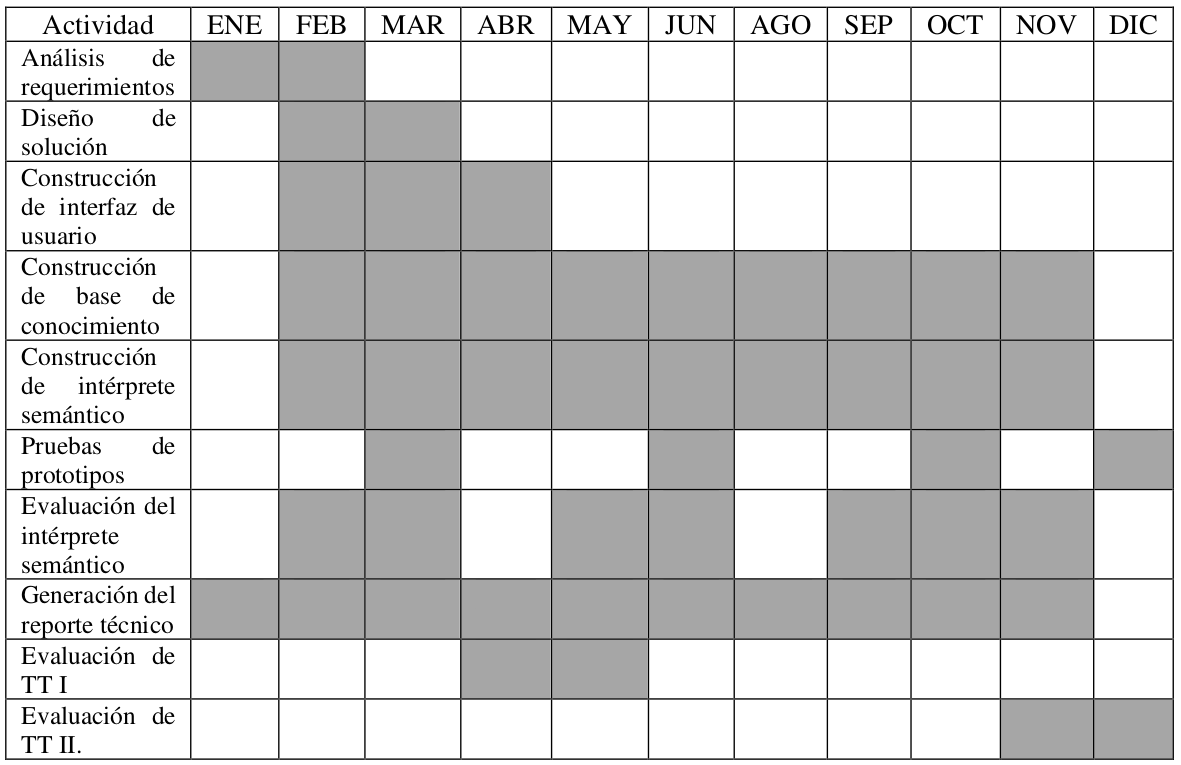
\includegraphics[scale=0.38]{images/4/cronograma}
    \caption{Cronograma de actividades para el desarrollo de este proyecto.}
    \label{fig:cronograma}
\end{figure}
